\documentclass[10pt]{article}
\usepackage[margin=.65in]{geometry}\usepackage{amsmath,amssymb,tikz,hyperref}
\setlength{\parindent}{0pt}\setlength{\parskip}{5pt}
\begin{document}
\textbf{Widened modular powers and generated inverse certificates}\hfill2026-10-31\\T-1154. Producer source-model proof; independent source-fidelity review pending.
\section*{Checked chain}
For arbitrary UInt64 operands, $ab<2^{128}$. The BitVec128 model of widening, multiplying, reducing and narrowing equals exact natural modular multiplication for positive modulus. Its remainder fits back into UInt64; this primitive needs no $p<2^{31}$ bound.

The binary-loop invariant is $r\,a^e$. Parity, right shift and skipped final squaring preserve it. The fuel theorem assumes $e<2^{\mathrm{fuel}}$, so 64 steps cover every UInt64 exponent. For $1<p$ and canonical base, the result is canonical and decodes to $a^e$.
\begin{center}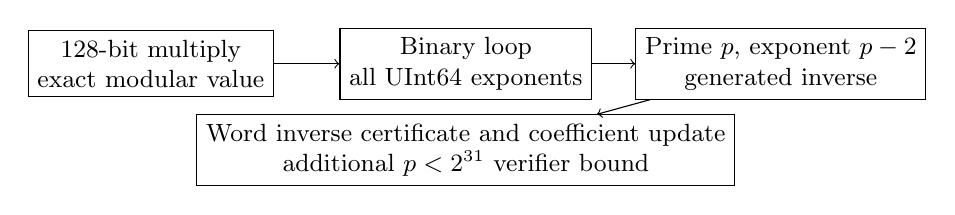
\begin{tikzpicture}[every node/.style={draw,align=center,font=\small}]
\node (a) at (0,0) {128-bit multiply\\exact modular value};
\node (b) at (4,0) {Binary loop\\all UInt64 exponents};
\node (c) at (8,0) {Prime $p$, exponent $p-2$\\generated inverse};
\node (d) at (4,-1.1) {Word inverse certificate and coefficient update\\additional $p<2^{31}$ verifier bound};
\draw[->](a)--(b);\draw[->](b)--(c);\draw[->](c)--(d);
\end{tikzpicture}\end{center}
For prime $p$ and nonzero canonical input, the standard finite-group-cardinality argument gives the inverse. Under $p<2^{31}$, its word product supplies the preceding InverseWitness. The composed coefficient-update theorem now uses this generated inverse.
\section*{Controls and readback}
Fourteen loop declarations, six inversion/composition declarations and eighteen controls receive 38 named axiom readbacks. Controls include inverse $2\mapsto9$ modulo 17, identity/negative-one inverses, exponents 0/1/$2^{64}-1$, zero base, maximum operands and the composed slot result.

The widened value $2^{63}\cdot2\bmod5$ is 1; narrow UInt64 multiplication gives 0. At composite $p=15,a=2$, exponent $p-2$ returns 2 and fails the inverse certificate. Zero modulus, modulus one and zero inversion input are excluded from their respective theorem domains.
\section*{Source and evidence}
Source excerpts/hashes bind \texttt{three\_leads.rs}:195--200,307--332,588--600. The source dispatch is odd-characteristic $n=1$ without diagnostic tables. BitVec128 models Rust u128 arithmetic; this is not compiled-binary equivalence. Full array-loop composition and geometric class transport remain separate bindings.

The first widened attempt needed the explicit ofNat conversion lemma; the first Fermat attempt needed an implicit argument instantiated. Corrected attempts and controls passed. Nonfatal deprecation warnings remain. Two exploratory cache planners failed import parsing; no cache was copied or built. Existing imported group-cardinality lemmas sufficed. Error summaries and native Lean receipts are retained separately.

Native exits, unchanged input hashes and standard-axiom readback accompany the inspected PDF, editable diagram, status JSON and custody. Existing compiled dependencies remain in the trust boundary.

Sources: \href{https://lean-lang.org/doc/reference/latest/Basic-Types/Bitvectors/}{Lean Bitvectors} and \href{https://leanprover-community.github.io/mathlib4_docs/Mathlib/FieldTheory/Finite/Basic.html}{Mathlib finite-field/Fermat identities}, compared with pinned source. No scientific campaign, enumeration, timing or cost ratio. Cohort and campaign limits unchanged.
\end{document}
